\todo[inline]{In this chapter, we will describe the background of this master thesis. It contains all pieces of information needed to understand the thesis, even without any knowledge of the field processed.
The background can be split between the two fields concerned by this master thesis. On the one hand, we have the background concerning the development of the application, related to the field of the software engineering. On the other hand, we can describe the background relative to the field of market gardening.}


\section{In market gardening}


\subsection{Daily life scenario}
Most farmers plan their cropping during winter\cite{planification-methodology}, when they have more time to think about what they want to grow this year. Planning the coming year has several advantages : 

\begin{itemize}
	\item Know in advance what amounts of seeds and fertilizers they will have to order
	\item Take the time to decide what to grow and in what quantities
	\item Look back at the previous year to see which vegetables were the most profitable and adjust cropping according to this experience.
	\item Gain time during the rush season by having clearly in mind what has to be done
	\item Organise the year to spread the work as most as possible (everything can not be seeded the same week)
\end{itemize}

While really useful, this planning part is not always done by the market gardeners. 

Once the work season has started, this planning has to be adapted to the reality on the ground.
The weather is the major factor of changes in the planning. Indeed, some seeding requires several days of dry weather followed by one day of rain for example. In the case of difficult weather (late frost, large humidity,...), whatever was the initial plan, the gardener will have to adapt his schedule to the weather.




\paragraph{Market gardening} A market gardener is someone who produces fruit and vegetables on a relatively small area. The difference between a farmer and a market gardener is principally in the type of final product. Where a farmer will produce more cereals, a market gardener is specialized in fruits and vegetables. We will use the term \emph{Truck farmers} for gardens that are cultivated with heavy machinery.  


\paragraph{Bed} A bed in a market garden is a surface of production, usually a line. It is used to divide the field in smaller cultivated areas. A representation of beds is shown on figure \ref{fig:beds}. Market gardener usually choose the width of their beds according to the width of the tools they are going to use.

\begin{figure}
    \centering
    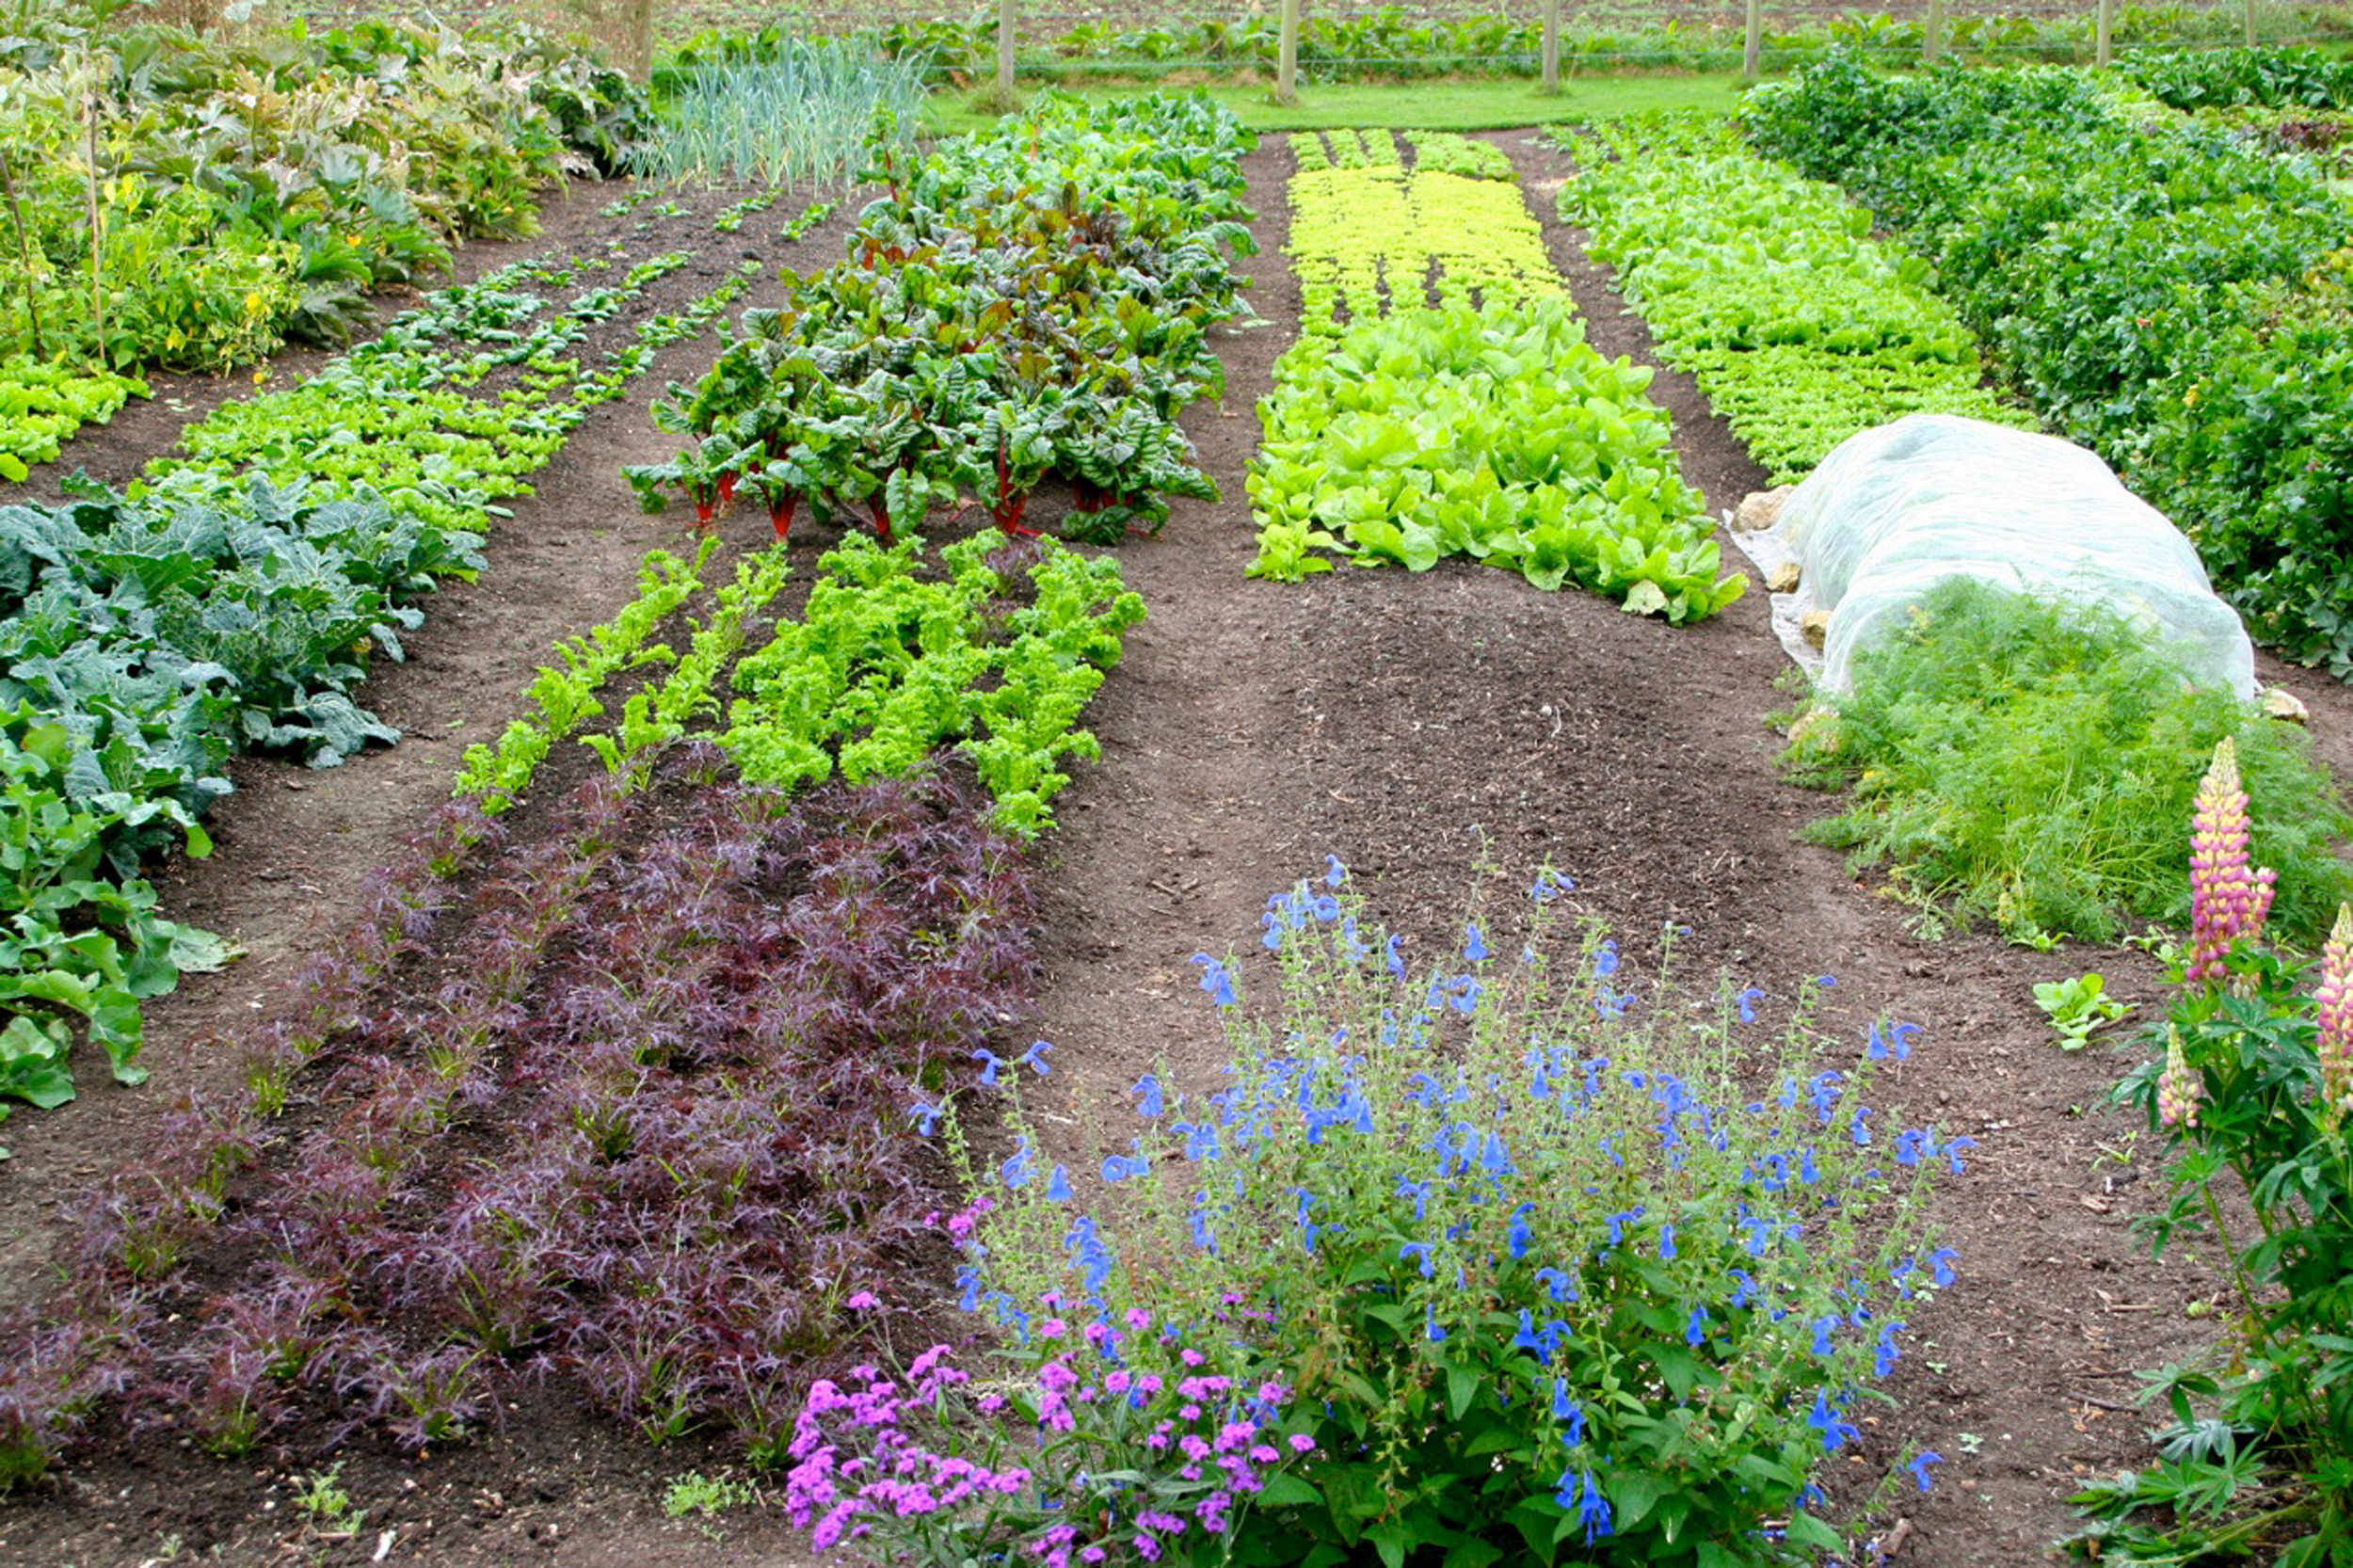
\includegraphics[width=0.6\textwidth]{images/beds.jpg}
    \caption{Beds in a market garden}
    \label{fig:beds}
\end{figure}

\paragraph{Crop rotation} In order to preserve the soil from draining and to eliminate some diseases specific to some plant species, some market gardener rotate their cropping. If they plant one type of vegetable on a bed, the year after they will plant another type of vegetable on this bed. They will not plant two years in a row the same vegetable on the same bed.

\paragraph{Work hours} Market gardeners don't count their hours as regular workers. They work all day in order to reach their objectives of the day. Most of them have no idea of how long each culture takes. It also means that they have no idea how profitable their cultures are. 

\paragraph{Planification} Market gardeners often plan during winter (when they have more time) what they are going to crop this year. However, day to day planning is not always easy. From our meetings with farmers, we have learn that it often happens that they have to stop what they are doing because they forgot to treat one of their cultures, for example. Of course, the degree of organisation depends on each market gardener.

\section{Link with this thesis?}

From our researchs, there are not lots of software to help farmers of all kind in their daily life. Most of them are not open source.

First, we found softwares like \emph{Mes petits légumes}\cite{mespetitslegumes} intended for non-professional market gardeners, with a great library of data about lots of vegetables. The software can be bought once for 19 \euro{} or one can use the free incomplete version.



Then, we have softwares like \emph{LEA}\cite{lea-agri} more focused on the management of the business and intended for big farms. Once again, the software is not open source and a subscription is required to use it.

Finally, we have found a software that seems to have a purpose and a target audience similar to this project. \emph{Tend}\cite{tend} is a software developed in the USA by a Startup.

These softwares show that farmers are in need of tools to help them in their planification and organisation. The poorness of softwares really adapted to their needs show that this field has been forgot by technology.

\todo[inline]{+ say that this is where this thesis comes in
Give more informations on each software. Screenshots. }